%% Creator: Inkscape 0.91, www.inkscape.org
%% PDF/EPS/PS + LaTeX output extension by Johan Engelen, 2010
%% Accompanies image file 'Strom_graf.pdf' (pdf, eps, ps)
%%
%% To include the image in your LaTeX document, write
%%   \input{<filename>.pdf_tex}
%%  instead of
%%   \includegraphics{<filename>.pdf}
%% To scale the image, write
%%   \def\svgwidth{<desired width>}
%%   \input{<filename>.pdf_tex}
%%  instead of
%%   \includegraphics[width=<desired width>]{<filename>.pdf}
%%
%% Images with a different path to the parent latex file can
%% be accessed with the `import' package (which may need to be
%% installed) using
%%   \usepackage{import}
%% in the preamble, and then including the image with
%%   \import{<path to file>}{<filename>.pdf_tex}
%% Alternatively, one can specify
%%   \graphicspath{{<path to file>/}}
%%
%% For more information, please see info/svg-inkscape on CTAN:
%%   http://tug.ctan.org/tex-archive/info/svg-inkscape
%%
\begingroup%
  \makeatletter%
  \providecommand\color[2][]{%
    \errmessage{(Inkscape) Color is used for the text in Inkscape, but the package 'color.sty' is not loaded}%
    \renewcommand\color[2][]{}%
  }%
  \providecommand\transparent[1]{%
    \errmessage{(Inkscape) Transparency is used (non-zero) for the text in Inkscape, but the package 'transparent.sty' is not loaded}%
    \renewcommand\transparent[1]{}%
  }%
  \providecommand\rotatebox[2]{#2}%
  \ifx\svgwidth\undefined%
    \setlength{\unitlength}{352.8bp}%
    \ifx\svgscale\undefined%
      \relax%
    \else%
      \setlength{\unitlength}{\unitlength * \real{\svgscale}}%
    \fi%
  \else%
    \setlength{\unitlength}{\svgwidth}%
  \fi%
  \global\let\svgwidth\undefined%
  \global\let\svgscale\undefined%
  \makeatother%
  \begin{picture}(1,0.42063368)%
    \put(0,0){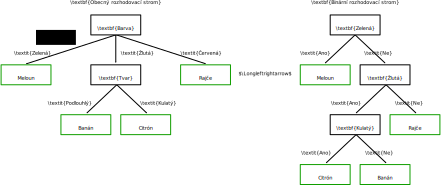
\includegraphics[width=\unitlength,page=1]{Strom_graf.pdf}}%
    \put(0.08049887,0.35260748){\color[rgb]{0,0,0}\makebox(0,0)[lt]{\begin{minipage}{0.09070295\unitlength}\raggedright \end{minipage}}}%
    \put(0.03514739,0.23922888){\color[rgb]{0,0,0}\makebox(0,0)[b]{\smash{}}}%
    \put(0.05782313,0.23922888){\color[rgb]{0,0,0}\makebox(0,0)[b]{\smash{Meloun}}}%
    \put(0.46598639,0.23922888){\color[rgb]{0,0,0}\makebox(0,0)[b]{\smash{Rajče}}}%
    \put(0.26190476,0.35260757){\color[rgb]{0,0,0}\makebox(0,0)[b]{\smash{\textbf{Barva}}}}%
    \put(0.80612245,0.35260757){\color[rgb]{0,0,0}\makebox(0,0)[b]{\smash{\textbf{Zelená}}}}%
    \put(0.80612245,0.12585034){\color[rgb]{0,0,0}\makebox(0,0)[b]{\smash{\textbf{Kulatý}}}}%
    \put(0.94217687,0.12585034){\color[rgb]{0,0,0}\makebox(0,0)[b]{\smash{Rajče}}}%
    \put(0.73809524,0.23922888){\color[rgb]{0,0,0}\makebox(0,0)[b]{\smash{Meloun}}}%
    \put(0.87414966,0.23922888){\color[rgb]{0,0,0}\makebox(0,0)[b]{\smash{\textbf{Žlutá}}}}%
    \put(0.27324263,0.29591822){\color[rgb]{0,0,0}\makebox(0,0)[lb]{\smash{\textit{Žlutá}}}}%
    \put(0.40929705,0.29591822){\color[rgb]{0,0,0}\makebox(0,0)[lb]{\smash{\textit{Červená}}}}%
    \put(0.11451247,0.29591822){\color[rgb]{0,0,0}\makebox(0,0)[rb]{\smash{\textit{Zelená}}}}%
    \put(0.89029284,0.29591822){\color[rgb]{0,0,0}\makebox(0,0)[rb]{\smash{\textit{Ne}}}}%
    \put(0.74943311,0.29591822){\color[rgb]{0,0,0}\makebox(0,0)[rb]{\smash{\textit{Ano}}}}%
    \put(0.31780186,0.18253857){\color[rgb]{0,0,0}\makebox(0,0)[lb]{\smash{\textit{Kulatý}}}}%
    \put(0.20748239,0.18253857){\color[rgb]{0,0,0}\makebox(0,0)[rb]{\smash{\textit{Podlouhlý}}}}%
    \put(0.60090772,0.24943296){\color[rgb]{0,0,0}\makebox(0,0)[b]{\smash{$\Longleftrightarrow$}}}%
    \put(0.26190476,0.41156559){\color[rgb]{0,0,0}\makebox(0,0)[b]{\smash{\textbf{Obecný rozhodovací strom}}}}%
    \put(0.80612286,0.41156559){\color[rgb]{0,0,0}\makebox(0,0)[b]{\smash{\textbf{Binární rozhodovací strom}}}}%
    \put(0.19387755,0.12585034){\color[rgb]{0,0,0}\makebox(0,0)[b]{\smash{Banán}}}%
    \put(0.32993197,0.12585034){\color[rgb]{0,0,0}\makebox(0,0)[b]{\smash{Citrón}}}%
    \put(0.26190476,0.23922916){\color[rgb]{0,0,0}\makebox(0,0)[b]{\smash{\textbf{Tvar}}}}%
    \put(0.96058707,0.18253857){\color[rgb]{0,0,0}\makebox(0,0)[rb]{\smash{\textit{Ne}}}}%
    \put(0.81972727,0.18253857){\color[rgb]{0,0,0}\makebox(0,0)[rb]{\smash{\textit{Ano}}}}%
    \put(0.73809524,0.01247165){\color[rgb]{0,0,0}\makebox(0,0)[b]{\smash{Citrón}}}%
    \put(0.87414966,0.01247165){\color[rgb]{0,0,0}\makebox(0,0)[b]{\smash{Banán}}}%
    \put(0.89255986,0.0691603){\color[rgb]{0,0,0}\makebox(0,0)[rb]{\smash{\textit{Ne}}}}%
    \put(0.75170006,0.0691603){\color[rgb]{0,0,0}\makebox(0,0)[rb]{\smash{\textit{Ano}}}}%
  \end{picture}%
\endgroup%
